\documentclass[modern]{aastex61}

% All the packages
%\usepackage[letterpaper]{geometry}
\usepackage{microtype}
\usepackage{url}
\usepackage{amsmath}
\usepackage{mathtools}
\usepackage{esint}
\usepackage{amssymb}
\usepackage{natbib}
\usepackage{multirow}
\usepackage{graphicx}
\usepackage{scalerel}
\usepackage{calc}
\usepackage{etoolbox}
\usepackage{marginnote}
\usepackage{nicefrac}
\usepackage{tabstackengine}
\usepackage{diagbox}
\usepackage[makeroom]{cancel}
\usepackage{mathdots}
\usepackage{bbm}
\usepackage{booktabs}
\usepackage{xspace}
\stackMath

% Bibliography stuff
\bibliographystyle{aasjournal}

% Shorthand for this paper
\newcommand{\starry}{\textsf{starry}\xspace}

% References to text content
\newcommand{\documentname}{\textsl{article}}
\newcommand{\figureref}[1]{\ref{fig:#1}}
\newcommand{\Figure}[1]{Figure~\figureref{#1}}
\newcommand{\figurelabel}[1]{\label{fig:#1}}
\renewcommand{\eqref}[1]{\ref{eq:#1}}
\newcommand{\Eq}[1]{Equation~(\eqref{#1})}
\newcommand{\eq}[1]{\Eq{#1}}
\newcommand{\eqalt}[1]{Equation~\eqref{#1}}
\newcommand{\eqlabel}[1]{\label{eq:#1}}

% Add script hyperlinks as margin notes
\definecolor{proofcolor}{rgb}{0.1216,0.4667,0.7059}
\newcommand{\python}[1]{\marginnote{\href{https://github.com/rodluger/starry/tree/master/tex/figures/#1.py}{
\includegraphics[width=0.9cm]{figures/python.png}}}}
\newcommand{\mathematica}[1]{\marginnote{\href{https://github.com/rodluger/starry/tree/master/tex/notebooks/#1.nb}{
\includegraphics[width=0.6cm]{figures/mathematica.png}}}}
\newcommand{\todoproof}{\marginnote{\href{}{
\includegraphics[width=0.4cm]{figures/todo.png}}}}
\newcommand{\todo}[2]{\marginnote{\color{red}\textbf{#1:}\\\scriptsize\textbf{#2}}}

% Force margin notes to always be on the right side
% https://tex.stackexchange.com/a/69624

% Math stuff
\newcommand{\ii}{\ensuremath{\mathbf{i}}}
\newcommand{\T}{\ensuremath{\mathrm{T}}}
\newcommand{\dd}{\ensuremath{ \mathrm{d}}}
\newcommand{\unit}[1]{{\ensuremath{\mathrm{#1}}}}
\newcommand{\bvec}[1]{{\ensuremath{\mathbf{#1}}}}
\newcommand{\avec}[1]{{\ensuremath{\vec{\mathbf{#1}}}}}
\newcommand{\x}{\ensuremath{\mbox{$x$}}}
\newcommand{\y}{\ensuremath{\mbox{$y$}}}
\newcommand{\z}{\ensuremath{\mbox{$z$}}}
\newcommand{\xhat}{\ensuremath{\mathbf{\hat{x}}}}
\newcommand{\yhat}{\ensuremath{\mathbf{\hat{y}}}}
\newcommand{\zhat}{\ensuremath{\mathbf{\hat{z}}}}
\DeclareMathAlphabet\mathbfcal{OMS}{cmsy}{b}{n}
\DeclareMathOperator{\Tr}{Tr}
\DeclarePairedDelimiter\ceil{\lceil}{\rceil}
\DeclarePairedDelimiter\floor{\lfloor}{\rfloor}
\definecolor{dim}{rgb}{0.8,0.8,0.8}
\newcolumntype{L}[1]{>{\raggedright\let\newline\\\arraybackslash\hspace{0pt}}m{#1}}
\setcounter{MaxMatrixCols}{20}
\newcommand{\sinphi}{\ensuremath{\mbox{$u$}}}
\newcommand{\sinlambda}{\ensuremath{\mbox{$v$}}}
\newcommand{\bigdot}{\scaleto{\cdot}{6pt}}

% Bases
\newcommand{\pbasis}{\ensuremath{\bvec{\tilde{p}}}}
\newcommand{\gbasis}{\ensuremath{\bvec{\tilde{g}}}}
\newcommand{\ybasis}{\ensuremath{\bvec{\tilde{y}}}}
\newcommand{\pbasisn}{\ensuremath{\tilde{p}_n}}
\newcommand{\gbasisn}{\ensuremath{\tilde{g}_n}}
\newcommand{\ybasisn}{\ensuremath{\tilde{y}_n}}
\newcommand{\AOne}{\ensuremath{\bvec{A_1}}}
\newcommand{\ATwo}{\ensuremath{\bvec{A_2}}}

% Code examples
\usepackage{listings}
\definecolor{codegreen}{rgb}{0,0.6,0}
\definecolor{codegray}{rgb}{0.5,0.5,0.5}
\definecolor{codepurple}{rgb}{0.58,0,0.82}
\definecolor{backcolour}{rgb}{0.95,0.95,0.95}
\lstdefinestyle{mystyle}{
    backgroundcolor=\color{backcolour},
    commentstyle=\color{codegreen},
    keywordstyle=\color{magenta},
    numberstyle=\tiny\color{codegray},
    stringstyle=\color{codepurple},
    basicstyle=\small\ttfamily,
    breakatwhitespace=false,
    breaklines=true,
    captionpos=b,
    keepspaces=true,
    numbers=left,
    numbersep=5pt,
    showspaces=false,
    showstringspaces=false,
    showtabs=false,
    tabsize=2,
    aboveskip=1em,
    belowskip=1em
}
\lstset{style=mystyle}

% Inverse diagonal dots
\makeatletter
\def\Ddots{\mathinner{\mkern1mu\raise\p@
\vbox{\kern7\p@\hbox{.}}\mkern2mu
\raise4\p@\hbox{.}\mkern2mu\raise7\p@\hbox{.}\mkern1mu}}
\makeatother

% Typography obsessions
\setlength{\parindent}{3.0ex}
\renewcommand\quad{\hskip\fontdimen3\font}


\begin{document}\raggedbottom\sloppy\sloppypar\frenchspacing

\setlength{\abovedisplayskip}{1.5em}
\setlength{\belowdisplayskip}{1.5em}

\title{%
    \textbf{STARRY}: Analytic Occultation Light Curves
}

\author[0000-0002-0296-3826]{Rodrigo Luger}
\affil{Department~of~Astronomy, University~of~Washington, Seattle, WA}
\author{others}

\keywords{methods: analytical --- techniques: photometric}

\begin{abstract}
    We derive analytical, closed form solutions for the total flux
    emitted or reflected from a celestial body in the direction of
    an observer when the surface brightness map of the body is expressed
    as a sum of spherical harmonics.
    Our expressions apply to the computation of phase curves of stars and
    exoplanets, as well as to occultation light curves, including transits of
    planets across their host stars, occultations of planets by the star
    (secondary eclipses), and planet-planet and planet-moon occultations.
    We develop fast code in \textsc{C} that can be generally applied
    to any of these cases.
\end{abstract}

% ==============================================================================
% ------------------------------------------------------------------------------
% ------------------------------------------------------------------------------
%
\section{Introduction}
\label{sec:intro}
% ------------------------------------------------------------------------------
% ------------------------------------------------------------------------------
% ==============================================================================

Write a kick-ass intro here! \todo{write intro}

% ==============================================================================
% ------------------------------------------------------------------------------
% ------------------------------------------------------------------------------
\pagebreak
\section{Spherical Harmonics}
\label{sec:spharm}
% ------------------------------------------------------------------------------
% ------------------------------------------------------------------------------
% ==============================================================================

The real spherical harmonic $Y_{lm}(\theta,\phi)$ of order $l$ and degree $m$
is defined in spherical coordinates as
%
\begin{align}
    \label{eq:ylmtp}
    Y_{lm}(\theta, \phi) =
    \begin{cases}
        \bar{P}_{lm}(\cos\theta)\cos(m\phi) & \qquad m \geq 0 \\
        \bar{P}_{l|m|}(\cos\theta)\sin(|m|\phi) & \qquad m < 0 \quad,
    \end{cases}
\end{align}
%
where $\bar{P}_{lm}$ is the normalized associated Legendre function. On the
surface of the unit sphere, we have
%
\begin{align}
    \label{eq:xyz}
    \x &= \sin\theta \cos\phi \nonumber \\
    \y &= \sin\theta \sin\phi \nonumber \\
    \z &= \cos\theta \quad.
\end{align}
%
Expanding Equation~(\ref{eq:ylmtp}) using the multiple angle formula, we obtain
%
\begin{align}
    \label{eq:ylm0}
    Y_{lm}(\x, \y , \z) =
    \begin{cases}
        \bar{P}_{lm}(\z) C_m(\x, \y, \z) & m \geq 0 \\
        \bar{P}_{l|m|}(\z) S_{|m|}(\x, \y, \z) & m < 0 \quad ,
    \end{cases}
\end{align}
%
where
%
\begin{align}
    C_m(\x, \y, \z) &= \left(\frac{1}{\sqrt{1 - \z^2}}\right)^m
                 \sum_{j\, \mathrm{even}}^{m}
                 \left(-1\right)^\frac{j}{2}
                 \binom{m}{j}
                 \x^{m - j}
                 \y^j \nonumber \\
                 %
    S_m(\x, \y, \z) &= \left(\frac{1}{\sqrt{1 - \z^2}}\right)^m
                 \sum_{j\, \mathrm{odd}}^{m}
                 \left(-1\right)^\frac{j-1}{2}
                 \binom{m}{j}
                 \x^{m - j}
                 \y^j \quad,
                 \label{eq:ylmcs}
\end{align}
%
and $\binom{\scaleto{\cdot}{6pt}}{\scaleto{\cdot}{6pt}}$ is the binomial
coefficient. The normalized associated Legendre function is defined as
%
\begin{align}
    \label{eq:plm}
    \bar{P}_{lm}(\z) &= A_{lm} \left(\sqrt{1-\z^2}\right)^m
                       \frac{\dd^m}{\dd \z^m}
                       \left[
                       \frac{1}{2^l l!}
                       \frac{\dd^l}{\dd \z^l}
                       \left(
                       \z^2 - 1
                       \right)^l
                       \right] \quad,
\end{align}
%
where
%
\begin{align}
    \label{eq:alm}
    A_{lm} = \sqrt{\frac{(2 - \delta_{m0})(2l + 1)(l - m)!}{4\pi(l + m)!}}
             \quad.
\end{align}
%
Expanding out the $\z$ derivatives, we obtain
%
\begin{align}
    \label{eq:plm_exp}
    \bar{P}_{lm}(\z) &= A_{lm} \left(\sqrt{1-\z^2}\right)^m\sum_{k=0}^{l-m}
                       \frac{2^l \left(\frac{l + m + k - 1}{2}\right)!}
                            {k!(l-m-k)!
                             \left(\frac{-l + m + k - 1}{2}\right)!}
                       \z^k
                       \quad,
\end{align}
%
which we combine with the previous results to write
%
\begin{align}
    \label{eq:ylmxyz}
    Y_{lm}(\x, \y , \z) &=
    \begin{dcases}
        \sum_{j\, \mathrm{even}}^m\sum_{k=0}^{l-m}
        \left(-1\right)^{\frac{j}{2}}
        A_{lm}
        B_{lm}^{jk}
        \x^{m - j}
        \y^j
        \z^k
        \qquad & m \ge 0 \\
        %
        \sum_{j\, \mathrm{odd}}^{|m|}\sum_{k=0}^{l-|m|}
        \left(-1\right)^{\frac{j-1}{2}}
        A_{l|m|}
        B_{l|m|}^{jk}
        \x^{|m| - j}
        \y^j
        \z^k
        \qquad & m < 0
    \end{dcases}
\end{align}
%
where
%
\begin{align}
    \label{blmnk}
    B_{lm}^{jk} =
    \frac{2^l m! \left(\frac{l + m + k - 1}{2}\right)!}
         {j! k! (m - j)! (l - m - k)!
          \left(\frac{-l + m + k - 1}{2}\right)!} \quad.
\end{align}
%
\begin{figure}[t!]
    \begin{centering}
    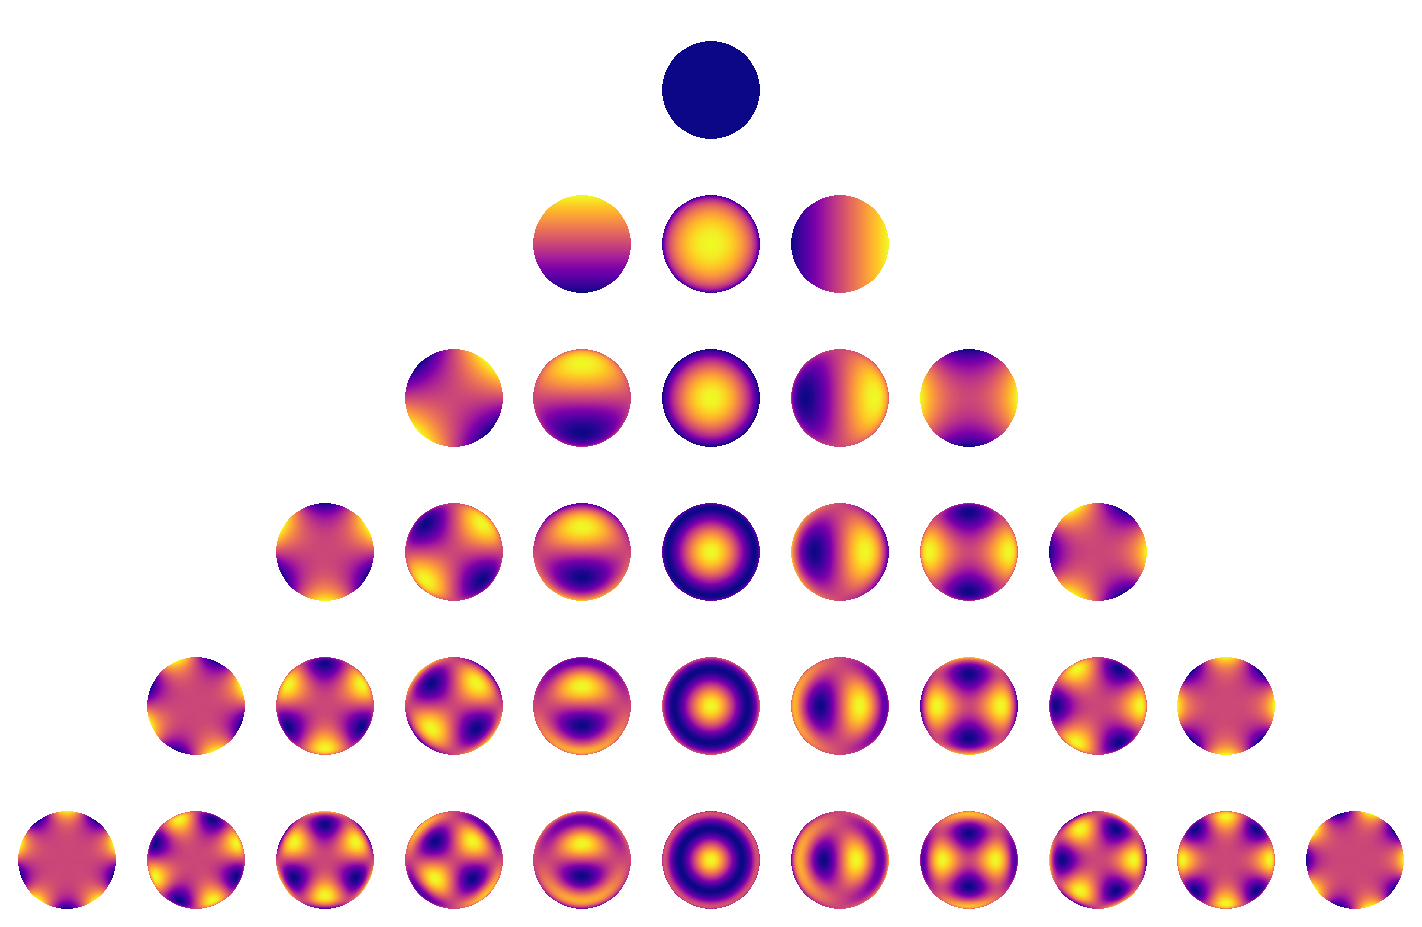
\includegraphics[width=\linewidth]{figures/ylms.pdf}
    \caption{\label{fig:ylms}
             \script{ylms}
             The real spherical harmonics up to order $l = 5$ computed from
             Equation~(\ref{eq:ylmxy}). In these plots, the $x$-axis points
             to the right, the $y$-axis points up, and the $z$-axis points
             out of the page. An animated version can be viewed
             \href{https://raw.githubusercontent.com/rodluger/%
                   cartograpy/gif/ylms.gif}{here}.}
    \end{centering}
\end{figure}
%
Since we are confined to the surface of the unit sphere, we have
$\z = \sqrt{1 - \x^2 - \y^2}$ and we may expand $\z^k$ using
the binomial theorem:
%
\begin{align}
    \z^{k} &= (1 - \x^2 - \y^2)^\frac{k}{2} \nonumber \\[0.5em]
          &=
          \begin{dcases}
              \sum_{p\,\mathrm{even}}^{k}
              \sum_{q\,\mathrm{even}}^p
              (-1)^\frac{p}{2}
              C_{pq}^{k}
              \x^{p-q} \y^{q}
              \qquad & k\,\mathrm{even} \\
              %
              \sum_{p\,\mathrm{even}}^{k - 1}
              \sum_{q\,\mathrm{even}}^p
              (-1)^\frac{p}{2}
              C_{pq}^{k-1}
              \x^{p-q} \y^{q} \sqrt{1 - \x^2 - \y^2}
              \qquad & k\,\mathrm{odd} \quad,
          \end{dcases}
          \label{eq:zk}
\end{align}
%
where
%
\begin{align}
    \label{eq:ckpq}
    C_{pq}^{k} =
    \frac{\left(\frac{k}{2}\right)!}{\left(\frac{q}{2}\right)!
    \left(\frac{k-p}{2}\right)! \left(\frac{p-q}{2}\right)!} \quad.
\end{align}
%
This gives us an expression for the spherical harmonic $Y_{lm}$
as a function of $\x$ and $\y$ only:
%
\begin{align}
    \label{eq:ylmxy}
    Y_{lm}(\x, \y) &=
    \begin{dcases}
        \!\begin{aligned}%[b]
            &
                \sum_{j\, \mathrm{even}}^m
                \sum_{k\, \mathrm{even}}^{l-m}
                \sum_{p\,\mathrm{even}}^{k}
                \sum_{q\,\mathrm{even}}^p
                \left(-1\right)^{\frac{j+p}{2}}
                A_{lm}
                B_{lm}^{jk}
                C_{pq}^{k}
                \x^{m - j + p - q}
                \y^{j + q}
            \, + \\
            &
                \sum_{j\, \mathrm{even}}^m
                \sum_{k\, \mathrm{odd}}^{l-m}
                \sum_{p\,\mathrm{even}}^{k - 1}
                \sum_{q\,\mathrm{even}}^p
                \left(-1\right)^{\frac{j+p}{2}}
                A_{lm}
                B_{lm}^{jk}
                C_{pq}^{k - 1}
                \x^{m - j + p - q}
                \y^{j + q}
                \z
       \end{aligned}
       &
       \quad m \ge 0 \\
       %
       %
       \\
       %
       %
       \!\begin{aligned}%[b]
           &
               \sum_{j\, \mathrm{odd}}^{|m|}
               \sum_{k\, \mathrm{even}}^{l-|m|}
               \sum_{p\,\mathrm{even}}^{k}
               \sum_{q\,\mathrm{even}}^p
               \left(-1\right)^{\frac{j+p-1}{2}}
               A_{l|m|}
               B_{l|m|}^{jk}
               C_{pq}^{k}
               \x^{|m| - j + p - q}
               \y^{j + q}
           \, + \\
           &
               \sum_{j\, \mathrm{odd}}^{|m|}
               \sum_{k\, \mathrm{odd}}^{l-|m|}
               \sum_{p\,\mathrm{even}}^{k - 1}
               \sum_{q\,\mathrm{even}}^p
               \left(-1\right)^{\frac{j+p-1}{2}}
               A_{l|m|}
               B_{l|m|}^{jk}
               C_{pq}^{k - 1}
               \x^{|m| - j + p - q}
               \y^{j + q}
               \z
      \end{aligned}
      &
      \quad m < 0
   \end{dcases}
    %
\end{align}
%
where $\z = \z(\x, \y) = \sqrt{1 - \x^2 - \y^2}$.

% ==============================================================================
% ------------------------------------------------------------------------------
% ------------------------------------------------------------------------------
\pagebreak
\section{Surface Map Vectors}
\label{sec:vectors}
% ------------------------------------------------------------------------------
% ------------------------------------------------------------------------------
% ==============================================================================

We represent a surface map as a vector $\bvec{y}$ of spherical harmonic
coefficients such that the observed flux originating from the point
$(\x, \y)$ may be written
%
\begin{align}
    f(\x, \y) = \bvec{b_y}^\mathsf{T} \bvec{y}
    \quad,
\end{align}
%
where $\bvec{b_y} = \bvec{b_y}(\x, \y)$ is the basis of spherical harmonics,
arranged in increasing
degree and order:
%
\begin{align}
    \label{eq:by}
    \bvec{b_y} =
    \begin{pmatrix}
        Y_{0, 0} &
        Y_{1, -1} & Y_{1, 0} & Y_{1, 1} &
        Y_{2, -2} & Y_{2, -1} & Y_{2, 0} & Y_{2, 1} & Y_{2, 2} &
        \cdot\cdot\cdot
    \end{pmatrix}^\mathsf{T}
    \quad,
\end{align}
%
where $Y_{l, m} = Y_{l, m}(\x, \y)$ are given by \eq{ylmxy}.
For reference, in this basis the coefficient of the spherical harmonic
$Y_{l, m}$ is located at the index
%
\begin{align}
    n = l^2 + l + m
\end{align}
%
of the vector $\bvec{y}$. Conversely, the coefficient at index $n$
of $\bvec{y}$ corresponds
to the spherical harmonic of order and degree given by
%
\begin{align}
    \label{eq:lm}
    l &= \floor*{\sqrt{n}} \nonumber \\
    m &= n - \floor*{\sqrt{n}}^2 - \floor*{\sqrt{n}}
    \quad.
\end{align}
%

% ==============================================================================
% ------------------------------------------------------------------------------
% ------------------------------------------------------------------------------
\pagebreak
\section{Rotation}
\label{sec:rotation}
% ------------------------------------------------------------------------------
% ------------------------------------------------------------------------------
% ==============================================================================

% ------------------------------------------------------------------------------
\subsection{Euler Angles}
\label{sec:euler}
% ------------------------------------------------------------------------------

Defining a map as a vector of spherical harmonic coefficients makes it
straightforward to compute the projection of the map under arbitrary rotations
of the body via a rotation matrix $\bvec{R}$:
%
\begin{align}
    \label{eq:rotation}
    \bvec{y'} = \bvec{R} \, \bvec{y}
\end{align}
%
where $\bvec{y'}$ are the spherical harmonic coefficients of the rotated map.
\citet{AlvarezCollado1989} derived expressions for the rotation matrices for
the real spherical harmonics of a given order $l$ from the corresponding
complex rotation matrices \citep{Steinborn1973}:
%
\begin{align}
    \bvec{R}^l = \bvec{U}^{-1} \bvec{D}^l \bvec{U}
\end{align}
%
where
%
\begin{align}
    \label{eq:dl}
    \bvec{D}^l_{m,m'} &= \mathrm{e}^{-\ii (\alpha m' + \gamma m)}
                       (-1)^{m' + m}
                       \sqrt{
                            (l - m)! (l + m)! (l - m')! (l + m')!
                       }
                       \nonumber \\
                       & \phantom{=}
                       \times
                       \sum_k (-1)^k
                              \frac{
                                \cos\left(\frac{\beta}{2}\right)^{2l + m - m' - 2k}
                                \sin\left(\frac{\beta}{2}\right)^{-m + m' + 2k}
                              }{
                                k! (l + m - k)! (l - m' - k)! (m' - m + k)!
                              }
\end{align}
%
is the rotation matrix for the complex spherical harmonics of order $l$ and
%
\begin{equation}
    \setstackgap{L}{1.25\baselineskip}
    \fixTABwidth{T}
    \bvec{U} =
    \frac{1}{\sqrt{2}}
        \parenMatrixstack{
            \quad\quad\, \ddots \, \quad\quad\quad\quad
                   &     &     &     &          &     &     &     & \Ddots \\
                   & \ii &     &     &          &     &     &  1  &        \\
                   &     & \ii &     &          &     &  1  &     &        \\
                   &     &     & \ii &          &  1  &     &     &        \\
                   &     &     &     & \sqrt{2} &     &     &     &        \\
                   &     &     & \ii &          &  1  &     &     &        \\
                   &     & \ii &     &          &     &  1  &     &        \\
                   & \ii &     &     &          &     &     &  1  &        \\
            \Ddots &     &     &     &          &     &     &     & \ddots
        }\quad.
\end{equation}
%
describes the transformation from complex to real spherical harmonics. In
\eq{dl} above, $\alpha$, $\beta$, and $\gamma$ are the (proper) Euler angles
for rotation in the $z-y-z$ convention.
%
To obtain a rotation matrix for an arbitrary vector $\bvec{y}$ with spherical
harmonics of different orders up to $l = l_\mathrm{max}$, we define the
block-diagonal matrix $\bvec{R}$:
%
\begin{equation}
    \label{eq:rblockdiag}
    \setstackgap{L}{1.25\baselineskip}
    \fixTABwidth{T}
    \bvec{R} =
        \parenMatrixstack{
            \quad\quad \, \bvec{R}^0 \, \quad\quad
                       &            &            &            &  \\
                       & \bvec{R}^1 &            &            &  \\
                       &            & \bvec{R}^2 &            &  \\
                       &            &            & \bvec{R}^3 &  \\
                       &            &            &            & \ddots
        }\quad.
\end{equation}
%
Rotation of $\bvec{y}$ by the Euler angles $\alpha$, $\beta$, and $\gamma$
is performed via \eq{rotation} with $\bvec{R}$ given by \eq{rblockdiag}.

% ------------------------------------------------------------------------------
\subsection{Axis-angle}
\label{sec:axisangle}
% ------------------------------------------------------------------------------

It is often more convenient to define a rotation by an axis $\bvec{u}$
and an angle $\theta$ of rotation about that axis. Given a unit vector
$\bvec{u}$ and an angle $\theta$, we can find the corresponding Euler
angles by comparing the 3-dimensional Cartesian rotation matrices for
both systems,
%
\begin{equation}
    \label{eq:rotP}
    \setstackgap{L}{1.25\baselineskip}
    \fixTABwidth{T}
    \mathbf{P} =
        \parenMatrixstack{
        c_\theta + u_x^2 \left(1 - c_\theta\right)
        &
        u_x u_y \left(1 - c_\theta\right) - u_z s_\theta
        &
        u_x u_z \left(1 - c_\theta\right) + u_y s_\theta
        \\
        u_y u_x \left(1 - c_\theta\right) + u_z s_\theta
        &
        % Add a little padding
        \makebox[1.5em]{}
        c_\theta + u_y^2\left(1 - c_\theta\right)
        \makebox[1.5em]{}
        &
        u_y u_z \left(1 - c_\theta\right) - u_x s_\theta
        \\
        u_z u_x \left(1 - c_\theta\right) - u_y s_\theta
        &
        u_z u_y \left(1 - c_\theta\right) + u_x s_\theta
        &
        c_\theta + u_z^2\left(1 - c_\theta\right)
        }
\end{equation}
%
for axis-angle rotations and
%
\begin{equation}
    \label{rotQ}
    \setstackgap{L}{1.25\baselineskip}
    \fixTABwidth{T}
    \mathbf{Q} =
        \parenMatrixstack{
        c_\alpha c_\beta c_\gamma - s_\alpha s_\gamma
        &
        -c_\gamma s_\alpha - c_\alpha c_\beta s_\gamma
        &
        c_\alpha s_\beta
        \\
        c_\alpha s_\gamma + c_\beta c_\gamma s_\alpha
        &
        c_\alpha c_\gamma - c_\beta s_\alpha s_\gamma
        &
        s_\alpha s_\beta
        \\
        -c_\gamma s_\beta
        &
        s_\beta s_\gamma
        &
        \makebox[4.2em]{}
        c_\beta
        \makebox[4.2em]{}
        }\quad,
\end{equation}
%
for Euler rotations,
where $c_{\scaleto{\cdot}{6pt}} \equiv \cos(\cdot)$
and $s_{\scaleto{\cdot}{6pt}} \equiv \sin(\cdot)$.
Comparison of the two matrices gives us expressions for the Euler
angles in terms of $\bvec{u}$ and $\theta$:
%
\begin{align}
    \label{eq:eulerangles}
    \begin{matrix}
        \cos\alpha = \frac{P_{0,2}}{\sqrt{P_{0,2}^2 + P_{1,2}^2}}
        & & & &
        \cos\beta = P_{3,3}
        & & & &
        \cos\gamma = -\frac{P_{2,0}}{\sqrt{P_{2,0}^2 + P_{2,1}^2}}
        \\
        \sin\alpha = \frac{P_{1,2}}{\sqrt{P_{0,2}^2 + P_{1,2}^2}}
        & & & &
        \sin\beta = \sqrt{1 - P_{3,3}^2}
        & & & &
        \sin\gamma = \frac{P_{2,1}}{\sqrt{P_{2,0}^2 + P_{2,1}^2}}
    \end{matrix}
    \quad.
\end{align}
%
Thus, given a spherical harmonic vector $\bvec{y}$, we can calculate
how it transforms under rotation by an angle $\theta$ about an axis $\bvec{u}$
by first computing the Euler angles (Equation~\ref{eq:eulerangles}) and using
those to construct the spherical harmonic rotation matrix
(Equation~\ref{eq:rblockdiag}).

% ==============================================================================
% ------------------------------------------------------------------------------
% ------------------------------------------------------------------------------
\pagebreak
\section{Change of Basis}
\label{sec:basis}
% ------------------------------------------------------------------------------
% ------------------------------------------------------------------------------
% ==============================================================================

% ------------------------------------------------------------------------------
\subsection{Polynomial Basis}
\label{sec:polybasis}
% ------------------------------------------------------------------------------

In order to compute the occultation light curve for a body with a given surface
map $\bvec{y}$, it is convenient to first find its polynomial representation
$\bvec{p}$, which we express as a vector of coefficients in the
polynomial basis $\bvec{b_p}$:
%
\begin{align}
    \label{eq:bp}
    \bvec{b_p}_n &=
    \begin{dcases}
        \x^\frac{l-m}{2} \y^\frac{l+m}{2} & \qquad l+m \, \mathrm{even}
        \\
        \x^\frac{l-m-1}{2} \y^\frac{l+m-1}{2} \z & \qquad l+m \, \mathrm{odd}
    \end{dcases}
    \nonumber\\[0.5em]
    \bvec{b_p} &=
    \begin{pmatrix}
        1 &
        \x & \z & \y &
        \x^2 & \x\z & \x\y & \y\z & \y^2 &
        \cdot\cdot\cdot
    \end{pmatrix}^\mathsf{T}
    \quad,
\end{align}
%
with $l$ and $m$ given by \eq{lm}.
%
%
As before, given $\bvec{p}$, the flux emitted from the point $(\x, \y)$
may be computed as
%
\begin{align}
    f(\x, \y) = \bvec{b_p}^\mathsf{T} \bvec{p}
    \quad.
\end{align}
%
To find $\bvec{p}$ given $\bvec{y}$, we
introduce the change of basis matrix $\bvec{A_1}$, which transforms
a vector in the spherical harmonic basis $\bvec{b_y}$ to the
polynomial basis $\bvec{b_p}$:
%
\begin{align}
    \bvec{p} = \bvec{A_1} \bvec{y}
\end{align}
%
The columns of $\bvec{A_1}$ are simply the polynomial vectors
corresponding to each of the spherical harmonics in \eq{by}. From
Equations (\ref{eq:ylmxy}) and (\ref{eq:bp}), we can calculate
the first few spherical harmonics and their corresponding polynomial vectors:
%
\begin{equation}
\def\arraystretch{1.3}
\begin{array}{@{}lcccccccl@{}}
    \phantom{..}
    Y_{0,0} = \frac{1}{2\sqrt{\pi}}
    & & & & & & & &
    \bvec{p}_0 = \frac{1}{2\sqrt{\pi}}
                  \begin{pmatrix}
                        1 & 0 & 0 & 0 & \cdot\cdot\cdot
                  \end{pmatrix}^\mathsf{T}
    %
    \\
    %
    Y_{1,-1} = \frac{\sqrt{3}}{2\sqrt{\pi}}\y
    & & & & & & & &
    \bvec{p}_1 = \frac{1}{2\sqrt{\pi}}
                  \begin{pmatrix}
                        0 & 0 & 0 & \sqrt{3} & \cdot\cdot\cdot
                  \end{pmatrix}^\mathsf{T}
    %
    \\
    %
    \phantom{..}
    Y_{1,0} = \frac{\sqrt{3}}{2\sqrt{\pi}}\z
    & & & & & & & &
    \bvec{p}_2 = \frac{1}{2\sqrt{\pi}}
                \begin{pmatrix}
                      0 & 0 & \sqrt{3} & 0 & \cdot\cdot\cdot
                \end{pmatrix}^\mathsf{T}
    %
    \\
    %
    \phantom{..}
    Y_{1,1} = \frac{\sqrt{3}}{2\sqrt{\pi}}\x
    & & & & & & & &
    \bvec{p}_3 = \frac{1}{2\sqrt{\pi}}
                  \begin{pmatrix}
                        0 & \sqrt{3} & 0 & 0 & \cdot\cdot\cdot
                  \end{pmatrix}^\mathsf{T}
    %
    \\
    %
    Y_{2,-2} = \cdot\cdot\cdot
    & & & & & & & &
    \bvec{p}_4 = \cdot\cdot\cdot
\end{array}
\end{equation}
%
From these we can construct $\bvec{A_1}$. As an example, for spherical
harmonics up to order $l_\mathrm{max} = 3$, this is
%
\begin{equation}
    \setstackgap{L}{1.25\baselineskip}
    \fixTABwidth{T}
    \bvec{A_1} =
    \frac{1}{2 \sqrt{\pi }}
        \parenMatrixstack{
            1 & 0 & 0 & 0 & 0 & 0 & \sqrt{5} & 0 & 0 \\
            0 & 0 & 0 & \sqrt{3} & 0 & 0 & 0 & 0 & 0 \\
            0 & 0 & \sqrt{3} & 0 & 0 & 0 & 0 & 0 & 0 \\
            0 & \sqrt{3} & 0 & 0 & 0 & 0 & 0 & 0 & 0 \\
            0 & 0 & 0 & 0 & 0 & 0 & -\frac{3 \sqrt{5}}{2} & 0 & \frac{\sqrt{15}}{2} \\
            0 & 0 & 0 & 0 & 0 & 0 & 0 & \sqrt{15} & 0 \\
            0 & 0 & 0 & 0 & \sqrt{15} & 0 & 0 & 0 & 0 \\
            0 & 0 & 0 & 0 & 0 & \sqrt{15} & 0 & 0 & 0 \\
            0 & 0 & 0 & 0 & 0 & 0 & -\frac{3 \sqrt{5}}{2} & 0 & -\frac{\sqrt{15}}{2}
        }\quad.
    \notebook{A1}
\end{equation}
%

% ------------------------------------------------------------------------------
\subsection{Greens Basis}
\label{sec:greensbasis}
% ------------------------------------------------------------------------------

As we will see in the next section, integrating the surface map over the disk of
the body is easier if we apply one final transformation to our input vector,
rotating it into what we will refer to as the \emph{Greens basis}, $\bvec{b_g}$:
%
\begin{align}
    \label{eq:bg}
    \bvec{b_g}_n &=
    \begin{dcases}
        %
        \frac{\mu+2}{2}\x^\frac{\mu}{2} \y^\frac{\nu}{2}
            & \qquad \nu \, \mathrm{even}
        \\[1em]
        %
        \z
            & \qquad \nu = \mu = 1
        \\[1em]
        %
        3\x^{l-2}\y\z
            & \qquad \nu \, \mathrm{odd}, \,
                     \mu = 1, \,
                     l \, \mathrm{even}
        \\[1em]
        %
        \z
        \bigg(
         -\x^{l-3} + \x^{l-1} + 4\x^{l-3}\y^2
        \bigg)
         & \qquad \nu \, \mathrm{odd}, \,
                  \mu = 1, \,
                  l \, \mathrm{odd}
        \\[1em]
        %
        \z
        \bigg(
            \frac{\mu-3}{2} \x^\frac{\mu-5}{2} \y^\frac{\nu-1}{2}
            -
            \frac{\mu-3}{2} \x^\frac{\mu-5}{2} \y^\frac{\nu+3}{2}
            -
            \frac{\mu+3}{2} \x^\frac{\mu-1}{2} \y^\frac{\nu-1}{2}
        \bigg)
            & \qquad \mathrm{otherwise}
    \end{dcases}
    \nonumber\\[1.5em]
    \bvec{b_g} &=
    \begin{pmatrix}
        1 &
        2\x & \z & \y &
        3\x^2 & -3\x\z & 2\x\y & 3\y\z & \y^2 &
        \cdot\cdot\cdot
    \end{pmatrix}^\mathsf{T}
    \quad,
\end{align}
%
where for convenience we define
%
\begin{align}
    \mu &= l - m \nonumber \\
    \nu &= l + m
    \quad
\end{align}
%
and the values of $l$ and $m$ are again given by \eq{lm}. Given
a polynomial vector $\bvec{p}$, the corresponding vector in
the Greens basis, $\bvec{g}$, can be found by performing another
change of basis operation:
%
\begin{align}
    \bvec{g} = \bvec{A_2} \bvec{p}
\end{align}
%
where the columns of the matrix $\bvec{A_2}$ are the Greens vectors
corresponding to each of the polynomial terms in \eq{bp}. In practice,
it is easier to express the elements of $\bvec{b_g}$ in terms
of the elements of $\bvec{b_p}$ and use those to populate the
columns of the matrix $\bvec{A_2}^{-1}$. Continuing our example
for $l_\mathrm{max} = 3$, our second change of basis matrix
is
%
\begin{equation}
    \setstackgap{L}{1.25\baselineskip}
    \fixTABwidth{T}
    \bvec{A_2} =
        \parenMatrixstack{
            \quad\quad\, 1\, \quad\quad\quad\quad & 0 & 0 & 0 & 0 & 0 & 0 & 0 & 0 \\
            0 & \frac{1}{2} & 0 & 0 & 0 & 0 & 0 & 0 & 0 \\
            0 & 0 & 1 & 0 & 0 & 0 & 0 & 0 & 0 \\
            0 & 0 & 0 & 1 & 0 & 0 & 0 & 0 & 0 \\
            0 & 0 & 0 & 0 & \frac{1}{3} & 0 & 0 & 0 & 0 \\
            0 & 0 & 0 & 0 & 0 & -\frac{1}{3} & 0 & 0 & 0 \\
            0 & 0 & 0 & 0 & 0 & 0 & \frac{1}{2} & 0 & 0 \\
            0 & 0 & 0 & 0 & 0 & 0 & 0 & \frac{1}{3} & 0 \\
            0 & 0 & 0 & 0 & 0 & 0 & 0 & 0 & 1
        }\quad.
    \notebook{A2}
\end{equation}
%
Given $\bvec{A_1}$ and $\bvec{A_2}$, we can easily transform a spherical harmonic
vector $\bvec{y}$ to a Greens vector $\bvec{g}$:
%
\begin{align}
    \bvec{g} &= \bvec{A_2} \bvec{A_1} \bvec{y} \nonumber \\
             &= \bvec{A} \, \bvec{y}
\end{align}
%
where $\bvec{A} = \bvec{A_2} \bvec{A_1}$ is the full change of basis matrix. For
$l_\mathrm{max} = 3$,
%
\begin{equation}
    \setstackgap{L}{1.25\baselineskip}
    \fixTABwidth{T}
    \bvec{A} =
        \frac{1}{2\sqrt{\pi}}
        \parenMatrixstack{
         1 & 0 & 0 & 0 & 0 & 0 & \frac{\sqrt{5}}{2} & 0 & 0 \\
         0 & 0 & 0 & \sqrt{3} & 0 & 0 & 0 & 0 & 0 \\
         0 & 0 & \sqrt{3} & 0 & 0 & 0 & 0 & 0 & 0 \\
         0 & \frac{\sqrt{3}}{2} & 0 & 0 & 0 & 0 & 0 & 0 & 0 \\
         0 & 0 & 0 & 0 & 0 & 0 & -\frac{3 \sqrt{5}}{4} & 0 & \frac{\sqrt{15}}{2} \\
         0 & 0 & 0 & 0 & 0 & 0 & 0 & \sqrt{\frac{5}{3}} & 0 \\
         0 & 0 & 0 & 0 & \sqrt{\frac{5}{3}} & 0 & 0 & 0 & 0 \\
         0 & 0 & 0 & 0 & 0 & -\sqrt{\frac{5}{3}} & 0 & 0 & 0 \\
         0 & 0 & 0 & 0 & 0 & 0 & -\frac{3 \sqrt{5}}{4} & 0 & -\frac{\sqrt{15}}{2}
        }\quad.
\end{equation}
%
For completeness, we note that the flux emitted from a given point on a map
described by the spherical harmonic vector $\bvec{y}$ is
%
\begin{align}
    \label{eq:fluxpoint}
    f(\x, \y) = \bvec{b_g}^\mathsf{T} \bvec{A} \, \bvec{y}
    \quad.
\end{align}
%

% ==============================================================================
% ------------------------------------------------------------------------------
% ------------------------------------------------------------------------------
\pagebreak
\section{Occultation Light Curves}
\label{sec:occultations}
% ------------------------------------------------------------------------------
% ------------------------------------------------------------------------------
% ==============================================================================

Consider a body of unit radius centered at the origin, with a surface map
given by the spherical harmonic vector $\bvec{y}$,
being occulted by a body of radius $r$ centered at the point $(x_0, y_0)$.
The total flux radiated
in the direction of the observer is obtained by integrating the surface
map over the visible portion of the occulted body's disk:
%
\begin{align}
    \label{eq:occint}
    F &=
    \oiint f(\x, \y) \, \dd \bvec{S}
    \nonumber \\
    &=
    \oiint \bvec{b_g}^\mathsf{T} (\x, \y) \bvec{A} \, \bvec{y} \, \dd \bvec{S}
    \nonumber \\
    &= \bvec{s}^\mathsf{T} \bvec{A} \, \bvec{y} \,
      \quad,
\end{align}
%
where we used \eq{fluxpoint} to express the flux in terms of our
map vector $\bvec{y}$ and we defined $\bvec{s}$ to be the column vector
whose $n^\mathrm{th}$ component is given by
%
\begin{align}
    \bvec{s}_n &\equiv
      \oiint \bvec{b_g}_n (\x, \y)  \, \dd \bvec{S}
    \quad.
\end{align}
%
In the equation above, the surface \bvec{S} over which the integral is taken
is a function of $r$, $x_0$, and $y_0$. In general, this integral is
difficult (and often impossible) to compute directly.
%
A clever workaround, introduced by \citet{Pal2012},
is to use Green's theorem to express this surface integral as the line integral
of a vector function $\avec{G}$ along the boundary of the same surface:
%
\begin{align}
    \label{eq:greens}
    \bvec{s}_n &=
    \oiint \bvec{b_g}_n (\x, \y) \, \dd \bvec{S}
    =
    \oint \bvec{G} (\x, \y) \cdot \dd \avec{r}
    \quad
\end{align}
%
where $\bvec{G} (\x, \y) = G_x (\x, \y) \, \xhat + G_y (\x, \y) \, \yhat$ is
chosen such that
%
\begin{align}
    \label{eq:DGL}
    \bvec{G} \wedge \bvec{F} = \bvec{b_g}_n(\x, \y)
    \quad.
\end{align}
%
The operation $\bvec{D} \wedge \bvec{G}$ denotes the
\emph{exterior derivative} of $\bvec{G}$. In two-dimensional Cartesian
coordinates, it is given by
%
\begin{align}
    \label{eq:extderiv}
    \bvec{D} \wedge \bvec{G} &\equiv \frac{\dd G_y}{\dd \x}
                                   - \frac{\dd G_x}{\dd \y} \quad.
\end{align}
%




%
%
\begin{figure}[p!]
    \begin{centering}
    \includegraphics[width=\linewidth]{figures/geometry.pdf}
    \caption{\label{fig:geometry}
             \script{geometry}
             Geometry of the occultation problem.
             The occulted body is centered
             at the origin and has unit radius, while the occultor
             is centered at $(x_0, y_0)$ and has radius $r$. We first rotate
             the two bodies about the origin through an angle
             $\theta = \nicefrac{\pi}{2} - \mathrm{arctan2}(y_0, x_0)$
             so the problem is symmetric about the $y$-axis. In this frame,
             the occultor is located at $(0, b)$, where
             $b = \sqrt{x_0^2 + y_0^2}$ is the impact parameter.
             The arc of the occultor
             that overlaps the occulted body (thick red curve) now extends from
             $\pi - \phi$ to $2\pi + \phi$, measured from the center of the
             occultor.
             The arc of the occulted body that is visible during
             the occultation (thick black curve) extends from
             $\pi - \lambda$ to $2\pi + \lambda$, measured from the origin.
             These are the curves along which the primitive integral
             (Equation~\ref{eq:primitive}) is evaluated.
             The angles $\phi$ and $\lambda$ are given by
             Equation~(\ref{eq:sinphi})
             and extend from $-\nicefrac{\pi}{2}$ to $\nicefrac{\pi}{2}$. When
             the occultor is completely within the disk of the occulted body,
             we define $\phi = \lambda = \nicefrac{\pi}{2}$.
             }
    \end{centering}
\end{figure}
%
%

We simplify the problem by performing a
rotation through an angle
$\theta = \nicefrac{\pi}{2} - \mathrm{arctan2}(y_0, x_0)$
about the $z$-axis ($\bvec{u} = \left[0, 0, 1\right]$)
so that the occultor lies along the
$+y$-axis, with its center located a distance $b = \sqrt{x_0^2 + y_0^2}$
from the origin (see Figure~\ref{fig:geometry}).
%
In this rotated frame, the limits of integration (the two points of intersection
between the occultor and the occulted body, should they exist)
are symmetric about the $y$-axis.
If we define $\phi \in [-\nicefrac{\pi}{2}, \, \nicefrac{\pi}{2}]$
as the angular position of the right hand side intersection point
relative to the occultor center, measured counter-clockwise
from the $+x$ direction, the arc of the occultor that overlaps the occulted
body extends from $\pi - \phi$ to $2\pi + \phi$ (see the Figure).
Similarly, defining $\lambda \in [-\nicefrac{\pi}{2}, \, \nicefrac{\pi}{2}]$
as the angular position of the same point relative to the origin, the
arc of the portion of the occulted body that is visible during the occultation
extends from $\pi - \lambda$ to $2\pi + \lambda$ (see the Figure).
%
With a little trig, it can be shown that
%
\begin{align}
    \label{eq:philam}
    \phi &=
    \begin{dcases}
        \arcsin{(\sinphi)}      & \qquad |1 - r| < b < 1 + r \\
        \frac{\pi}{2}           & \qquad b \le 1 - r
    \end{dcases}
    \nonumber \\
\intertext{and}
    \lambda &=
    \begin{dcases}
        \arcsin{(\sinlambda)}      & \qquad |1 - r| < b < 1 + r \\
        \frac{\pi}{2}              & \qquad b \le 1 - r
    \end{dcases}
\quad,
\end{align}
%
where we define
\begin{align}
    \begin{split}
        \sinphi &\equiv \frac{1 - r^2 - b^2}{2br}
    \end{split}
    \begin{split}
        \sinlambda &\equiv b + r \sinphi
    \end{split}
    \quad.
\end{align}
%
The case $b \le 1 - r$ corresponds to an occultation during which the occultor
is fully within the planet disk, so no points of intersection exist.
In this case,
we define $\phi$ such that the arc from $\pi - \phi$ to $2\pi + \phi$ spans the
entire circumference of the occultor, and $\lambda$ such that the arc
from $\pi - \lambda$ to $2\pi + \lambda$ spans the
entire circumference of the occulted body.
Note that if $b \ge 1 + r$, no occultation occurs, while
if $b \le r - 1$, the entire disk of the body is occulted and the total flux
is zero.

\bibliography{starry}

\end{document}
